\documentclass[11pt]{beamer}
\usetheme{Madrid}
\usefonttheme{serif}

\usepackage[utf8]{inputenc}
\usepackage[brazil]{babel}
\usepackage[T1]{fontenc}

\usepackage{amsmath}
\usepackage{amsfonts}
\usepackage{amssymb}
\usepackage{graphicx}

\DeclareMathOperator{\sen}{sen}
\DeclareMathOperator{\tg}{tg}

\setbeamertemplate{caption}[numbered]

\author[Autor]{Presenter:  Jingyuan Meng}
\title{Energy Conservation in Discrete Wavelet Transform (DWT) and Its Application to Image Compression}
% Informe o seu email de contato no comando a seguir
% Por exemplo, alcebiades.col@ufes.br
\newcommand{\email}{email}
%\setbeamercovered{transparent} 
\setbeamertemplate{navigation symbols}{} 
%\logo{} 

\date{2025.8.8}
%\subject{}

% ---------------------------------------------------------
% Selecione um estilo de referência
\bibliographystyle{apalike}

%\bibliographystyle{abbrv}
%\setbeamertemplate{bibliography item}{\insertbiblabel}
% ---------------------------------------------------------

% ---------------------------------------------------------
% Incluir os slides nos quais as referências foram citadas
%\usepackage[brazilian,hyperpageref]{backref}

%\renewcommand{\backrefpagesname}{Citado na(s) página(s):~}
%\renewcommand{\backref}{}
%\renewcommand*{\backrefalt}[4]{
%	\ifcase #1 %
%		Nenhuma citação no texto.%
%	\or
%		Citado na página #2.%
%	\else
%		Citado #1 vezes nas páginas #2.%
%	\fi}%
% ---------------------------------------------------------
\usepackage{amsmath}
\begin{document}

\begin{frame}
\titlepage
\end{frame}

\begin{frame}{outline}
\tableofcontents 
\end{frame}

\section{Research background and objectives}

\begin{frame}{Research background and objectives}
 \begin{block}{Advantages of Wavelet Transform}
    - Multiresolution analysis \\
    - frequency localization capability
    \end{block}
    
    \begin{block}{Importance of Energy Conservation}
    - Ensures information integrity in signal processing  \\
  - Theoretical basis for image compression, denoising
    \end{block}
    
    \begin{block}{Research Objectives}
    - Validate energy conservation mathematically  \\
  - Quantify energy retention via image compression experiments  
    \end{block}
\end{frame}

\section{Theoretical analysis}


\begin{frame}{Theoretical analysis}
  \begin{block}{Theoretical Foundations of DWT}
    \begin{itemize}
      \item Scaling function ($\phi$) and wavelet function ($\psi$)
      \item Multi-scale decomposition: Approximation ($cA$) and Detail   ($cH$, $cV$, $cD$) subbands
      \item Orthogonal Wavelet Basis Properties:
      \[
\langle \psi_{j,k},\,\psi_{m,n}\rangle
= \delta_{j,m}\,\delta_{k,n},
\qquad j,k,m,n\in\mathbb{Z}
\]


    \end{itemize}
  \end{block}



 

  \begin{block}{Critical Conditions}
    \begin{itemize}
      \item Use of orthogonal wavelets (e.g., Haar, Db1)
      \item No signal truncation or padding-induced errors
    \end{itemize}
  \end{block}
\end{frame}
\begin{frame}{ Energy Conservation Formula }
\begin{block}{Energy Conservation Formula for Orthogonal DWT}
    \begin{itemize}
    \item For orthogonal wavelet bases:
      \[
\sum_{i=1}^{M} \sum_{j=1}^{N} |x[i,j]|^2 = \sum_{k,l} |d_k[l]|^2 + \sum_{m} |a_J[m]|^2
\]  
\item For Haar wavelet bases:

     \[
     \begin{aligned}
\sum_{i,j} |x[i,j]|^2 =\sum_{i,j} |cA[i,j]|^2 + \sum_{i,j} |cH[i,j]|^2 \\+ \sum_{i,j} |cV[i,j]|^2 +\sum_{i,j} |cD[i,j]|^2
\end{aligned}
\]  
    \end{itemize}
  \end{block}



\end{frame}
\section{Experimental Design and Code Implementation}

\begin{frame}{Experimental Design and Code Implementation}
 \begin{block}{Workflow}
    \begin{itemize}
      \item Image preprocessing
      \begin{itemize}
           \item grayscale conversion
           \item resizing to power-of-2 dimensions
      \end{itemize}
      \item DWT decomposition("dwt2"function)
      \item Energy calculation and conservation validation
      \item Image reconstruction("idwt2"function)
    \end{itemize}
  \end{block}
\begin{block}{Parameters}
    \begin{itemize}
      \item Test image:"Lena"(52*52)
      \item Wavelet basis:Haar
    \end{itemize}
  \end{block}

\end{frame}

\begin{frame}{Code and Implementation}
    \begin{figure}
        \centering
        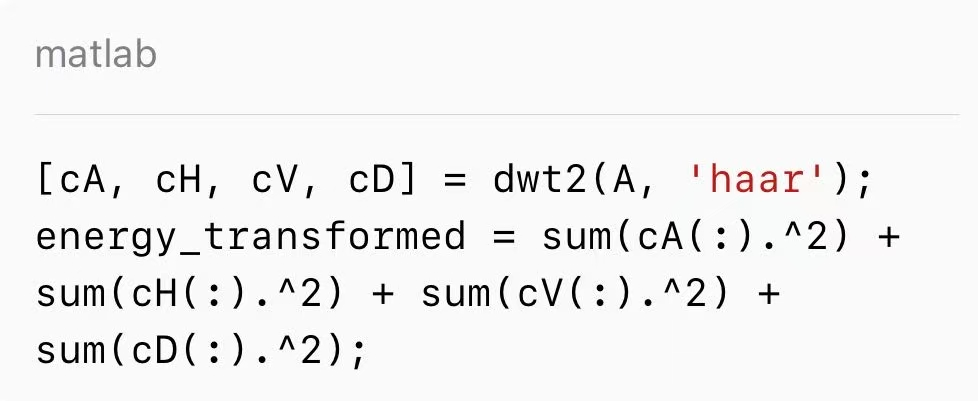
\includegraphics[width=0.5\linewidth]{代码2.jpg}
        \caption{"Haar"basis}
        \label{fig:placeholder}
    \end{figure}
    \begin{figure}
        \centering
        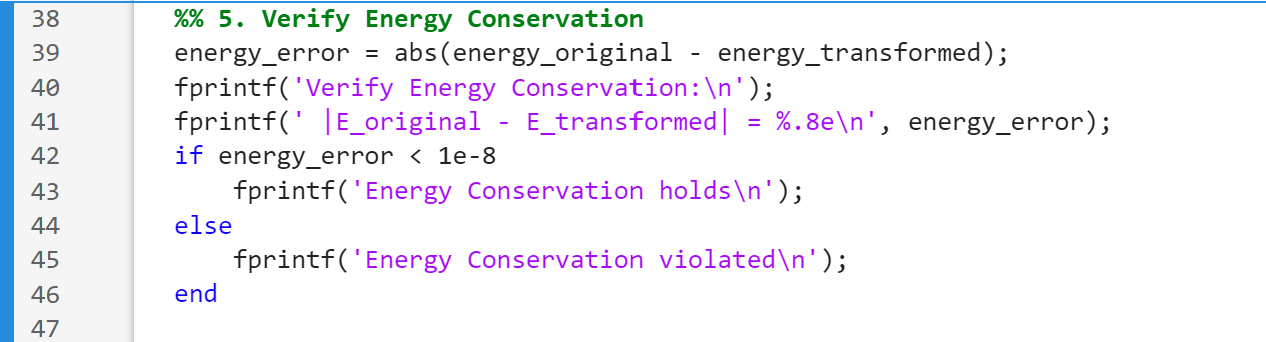
\includegraphics[width=1\linewidth]{代码3.png}
        \caption{Verify Energy Conservation}
        \label{fig:placeholder}
    \end{figure}
\end{frame}


\begin{frame}{Code and Implementation}
  \begin{figure}
      \centering
      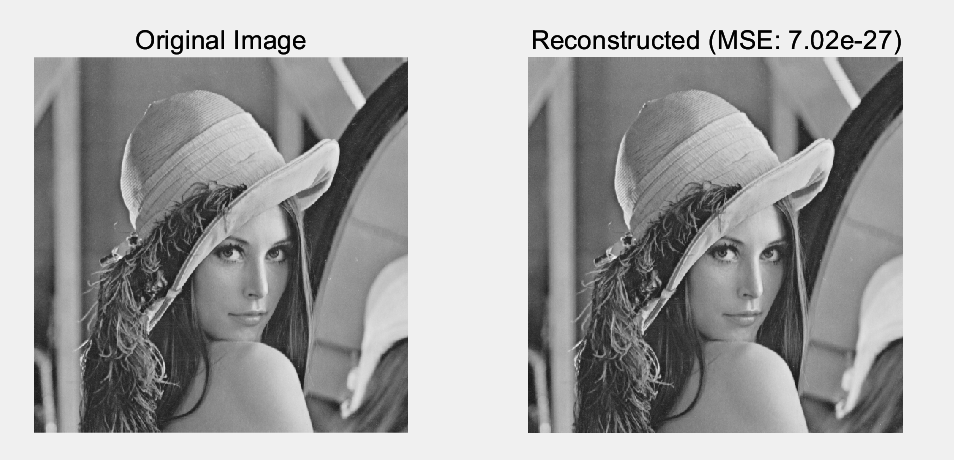
\includegraphics[width=0.5\linewidth]{图像1.png}
      
      \label{fig:placeholder}
  \end{figure}

  \begin{figure}
      \centering
      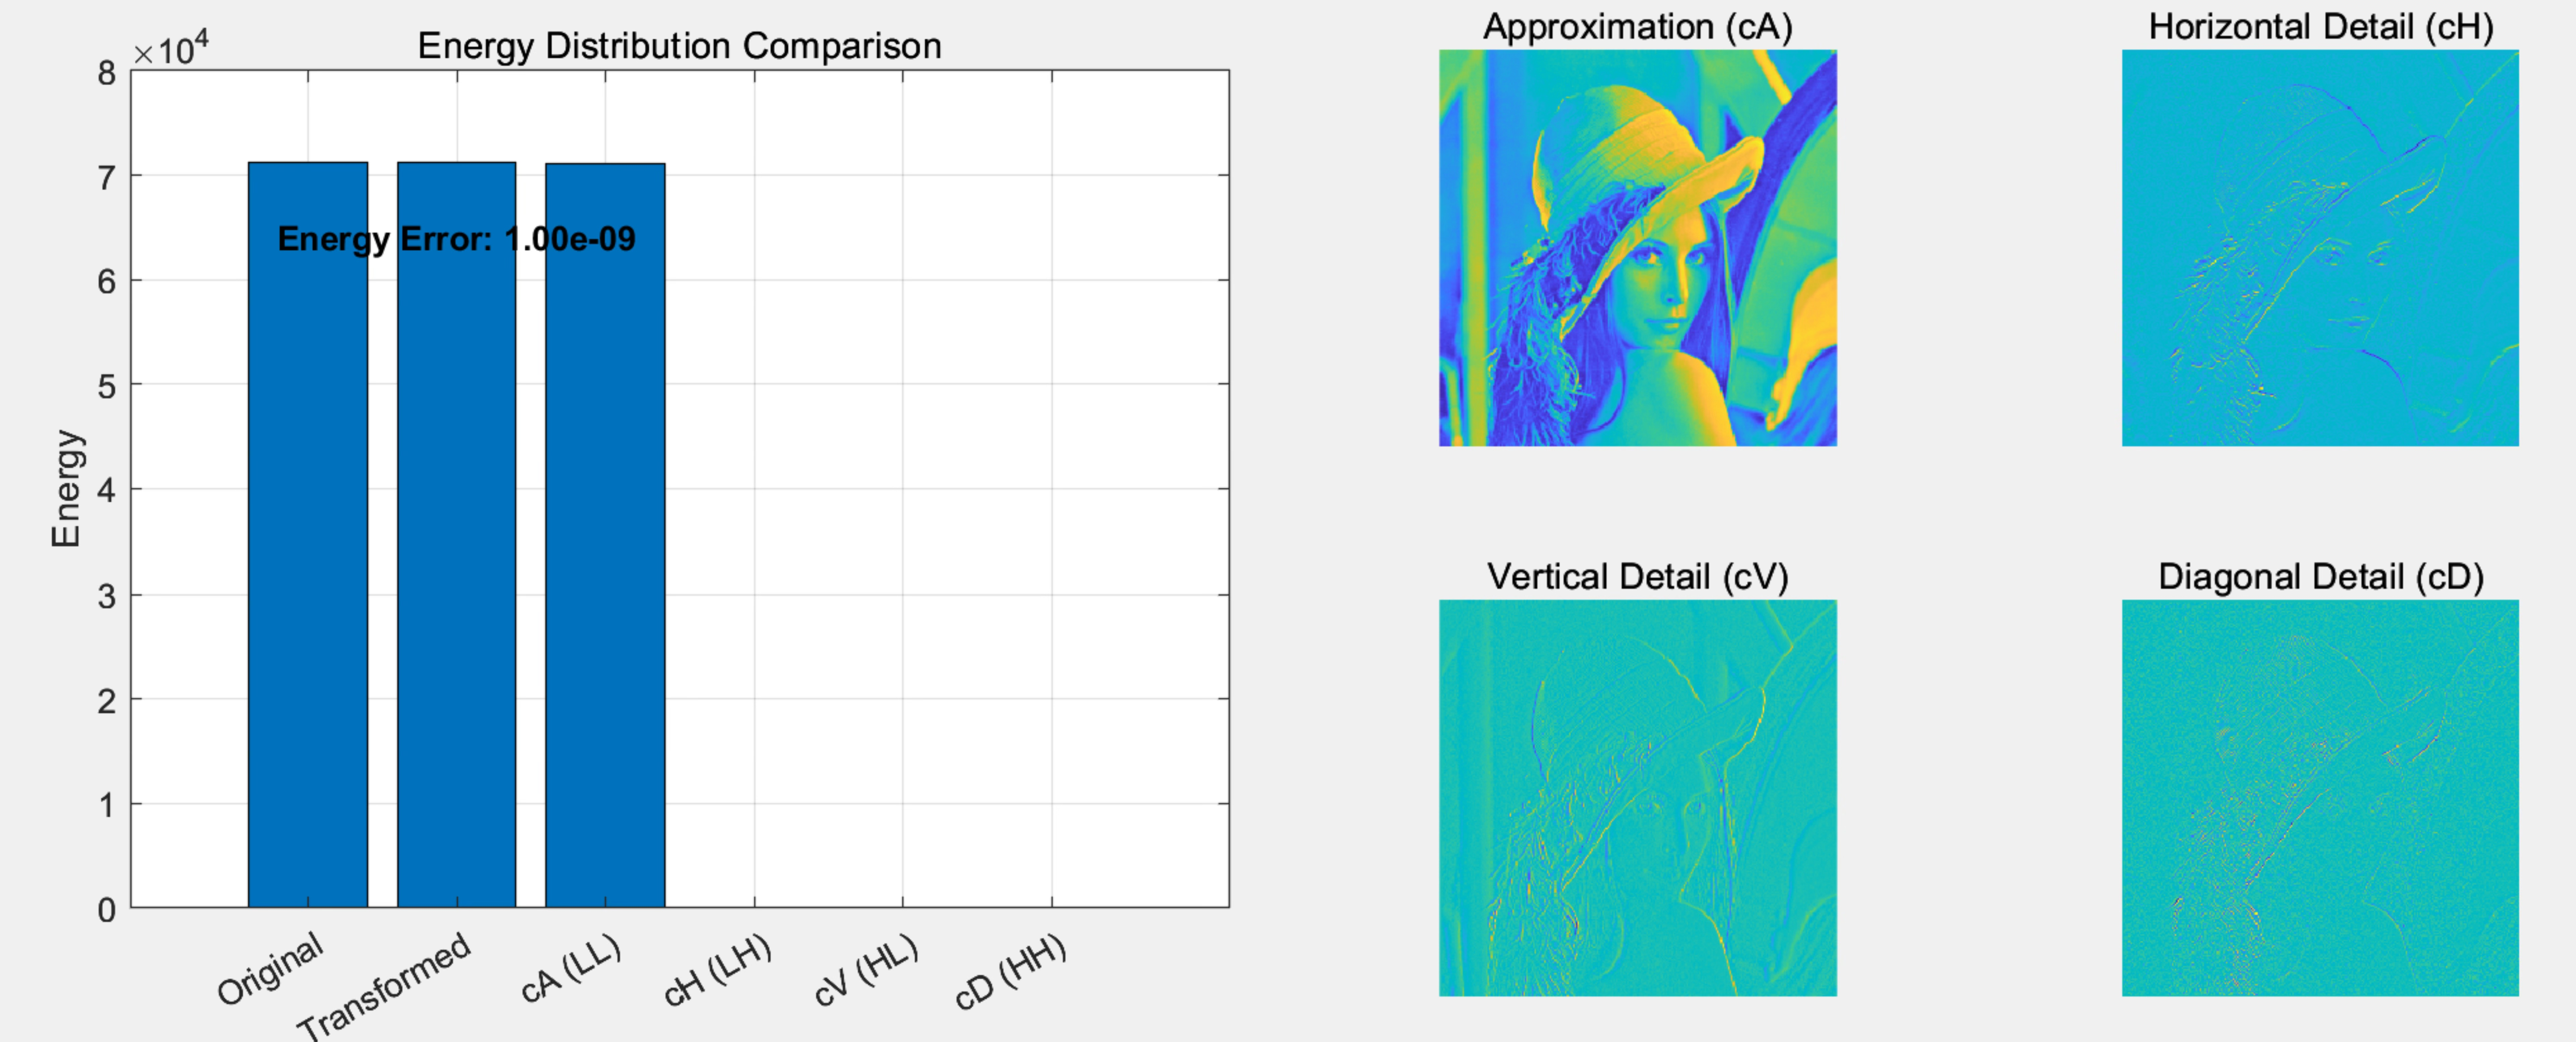
\includegraphics[width=0.75\linewidth]{图片4.jpg}
      
      \label{fig:placeholder}
  \end{figure}
\end{frame}

\section{Conclusions and Future Work}
\begin{frame}{Conclusions and Future Work}
 \begin{block}{Conclusions}
    \begin{itemize}
      \item DWT strictly satisfies energy conservation when using orthogonal wavelet bases  
      \item Proper image size alignment and orthogonal basis selection are critical factors  
      \end{itemize}
      \end{block}
      \begin{block}{Future Work}
    \begin{itemize}
      \item Energy error analysis for non-orthogonal wavelet frames  
      \item Study of energy distribution in multi-scale decomposition (multi-level DWT)   
      \end{itemize}
      \end{block}
    
\end{frame}


\end{document}